% das Papierformat zuerst
\documentclass[a4paper, 11pt]{article}
%more colors
\usepackage[dvipsnames]{xcolor}
% deutsche Silbentrennung
\usepackage[ngerman]{babel}
% wegen deutschen Umlauten
\usepackage[utf8]{inputenc}
% andere pdfs einbinden
\usepackage{pdfpages}
% um bilder einzubinden
\usepackage{graphicx}
% fuer source code listings
\usepackage{listings}
% seitenränder
\usepackage[left=3cm,right=3cm,top=2cm,bottom=2cm]{geometry}
% um hyperlinks einfügen zu können
\usepackage{hyperref}
% um weitere Symbole zu nutzen
\usepackage{amssymb}
% um weitere Operatoren zu nutzen
\usepackage{amsmath}
%Aufzaehlung
\usepackage{paralist}
%Beachtet, ob ein Leerzeichen syntaktisch passt oder nicht
\usepackage{xspace}
% um hyperlinks einfügen zu können
\usepackage{hyperref}
%um Kopf- und Fußzeile zu bearbeiten
\usepackage{fancyhdr}
%um Literaturverzeichnis auch im Inhaltsverzeichnis anzuzeigen
\usepackage{tocbibind}
%um Silbentrennungen angeben zu können, welche nicht unterstützt werden
\RequirePackage[ngerman=ngerman-x-latest]{hyphsubst}
%um Tabellen zu begrenzen, damit sie nicht in den Rand hineinragen
\usepackage{tabularx}
%um die landscape Umgebung zu nutzen (Querformat)
\usepackage{pdflscape}
%Stellt eine caption-Anweisung mit direkter Angabe des Gleitumgebungstyps bereit.
\usepackage{capt-of}
\usepackage{caption}

%ermöglicht Anführungsstriche unten und oben
\newcommand{\su}{\glqq} %unten
\newcommand{\so}{\grqq\xspace} %oben mit anschließendem Leerzeichen
\newcommand{\soo}{\grqq} %nur oben

%ermöglicht eckige Klammern
\newcommand{\eka}{$<$} %<
\newcommand{\ekz}{$>$\xspace} %> mit anschließendem Leerzeichen

%Versionsnummer
\newcommand{\version}{0.3}

% Tabellenabschnitt linksbündig
\newcommand{\ltab}{\raggedright\arraybackslash}
% Tabellenabschnitt zentriert
\newcommand{\ctab}{\centering\arraybackslash}
% Tabellenabschnitt rechtsbündig
\newcommand{\rtab}{\raggedleft\arraybackslash}

%Einstellungen für Fuß- und Kopfzeile
\pagestyle{fancy}
\fancyhf{}
\fancyhead[L]{\footnotesize M. Lüdemann $\cdot$ M. Butkereit $\cdot$ W. Schumacher $\cdot$ A. Melkonyan $\cdot$ M. Colbow $\cdot$ M. Cakir\\ Requirements and Design Documentation $\cdot$ ESEP WS2016(v\version) $\cdot$ HAW Hamburg}
%\fancyhead[C]{\footnotesize}
\fancyhead[R]{\footnotesize \today}
%\renewcommand{\headrulewidth}{0.0pt}
\fancyfoot[C]{\thepage}

%Stil des Literaturverzeichnisses bestimmen
\bibliographystyle{unsrt}

\begin{document}

% Den Titel festlegen
\title
{
    Requirements and Design Documentation\\
    \bigskip
    (RDD)\\
    \medskip
    {\normalsize Version \version}\\
    \bigskip
    ESEP - Praktikum - Wintersemester 2016
}

% Autor/en
\author
{
\begin{tabular}{llll}
Lüdemann&Mona&2212744&mona.luedemann1@haw-hamburg.de\\
Butkereit&Marvin&2247550&marvin.butkereit@haw-hamburg.de\\
Schumacher&Wilhelm&2245216&wilhelm.schumacher@haw-hamburg.de\\
Melkonyan&Anushavan&2243668&anushavan.melkonyan@haw-hamburg.de\\
Colbow&Marco&2177095&marco.colbow@haw-hamburg.de\\
Cakir&Mehmet&2195657&mehmet.cakir@haw-hamburg.de
\end{tabular}
}

% Erstelle die Titelseite
\maketitle

\noindent {\large Änderungshistorie:}
\begin{table}[h]
\begin{tabularx}{\textwidth}{|c|c|c|X|}
\hline
\textbf{Version} & \textbf{Author} & \textbf{Datum} & \centering\arraybackslash \textbf{Anmerkungen/Änderungen}\\
\hline
0.1&Mehmet Cakir&2016-10-18&Kapitel 1-4 und Testkonzept\\
\hline
0.2&Mehmet Cakir&2016-10-26&Korrekturen an Formulierung, Visualisierungen noch nicht festgelegt\\
\hline
0.3&Mehmet Cakir&2016-11-03&Testtabellen umformatiert. Tests zu Grundfunktionen, HAL\_UML, Systemgrenzen, Systemarchitektur und Visualisierungsentscheidung sowie entsprechend kurzen Text hinzugefügt.\\
\hline
0.4&Mehmet Cakir&2016-11-16&Neugliederung der Kapitel 4 und 7, Systemkontexte zusammengeführt, verwendete Werkzeuge ergänzt, Zeitmessung und FSM/HSM eingepflegt, diverse Umformulierungen.\\
\hline
\end{tabularx}
\label{changes}
\end{table}

\newpage

\tableofcontents

\newpage

\section{Teamorganisation}
Grundsätzlich kann jedes Teammitglied eine Aufgabe seiner Wahl übernehmen. Bei jedem Meeting werden die Aufgaben verteilt, worüber im folgenden Meeting über den Fortschritt diskutiert wird. Falls ein Mitglied seine Aufgabe fertiggestellt hat, übernimmt er eine Neue. Bei Nichteinhaltung des Zeitplans werden entsprechend der Zeitpuffer andere Aufgaben zurückgestellt. Die Aufgaben richten sich nach den zu bewältigenden Milestones(siehe \cite{esep}) zum jeweiligen Praktikumstermin. Für die Projektleitung und die Pflege des RDD-Dokuments wurde jeweils eine Person bestimmt, welche im Unterkapitel \ref{vantw} eingesehen werden können.

\subsection{Verantwortlichkeiten}\label{vantw}
\begin{table}[h]
\center
\begin{tabularx}{\textwidth}{|l|l|X|}
\hline
\textbf{Aufgabe}&\textbf{Zuständige/r}&\textbf{Bemerkung}\\
\hline
Projektleitung&Mona&Die Projektleitung überwacht den Projektfortschritt und benachrichtigt insbesondere bei Nichteinhalten des Zeitplans alle Teammitglieder. Außerdem hat die Projektleitung bei Unstimmigkeiten immer das letzte Wort. \\
\hline
RDD-Pflege&Mehmet&Der Zuständige ist für die Gestaltung und für die Vollständigkeit des RDDs verantwortlich. Er kann andere Gruppenmitglieder dazu auffordern Inhalte für das Dokument zu erarbeiten und ihm bereit zu stellen. \\
\hline 
Protkollführung&Alle Teammitglieder&Die Protokollführung wird reihum von Gruppenmitgliedern übernommen. Dabei wird folgende Reihenfolge eingehalten: $Mona\rightarrow Marvin\rightarrow Marco \rightarrow Wilhelm\rightarrow Mehmet\rightarrow Anushavan$ \\
\hline
\end{tabularx}
\caption{Zuteilung von Verantwortlichkeiten}
\label{labelname}
\end{table}

\subsection{Absprachen}
Zur Kommunikation außerhalb der Praktikumstermine werden Slack und WhatsApp verwendet. Unstimmigkeiten, Fragen und Inkenntnissetzung können somit interaktiv geklärt bzw. mitgeteilt werden. Es wird erwartet, dass jedes Teammitglied in einem Zeitfenster von 24 Stunden darauf reagiert. In folgender Abbildung \ref{meets} werden die Termine der Meetings dargestellt:
\begin{figure}[h]
\centering 
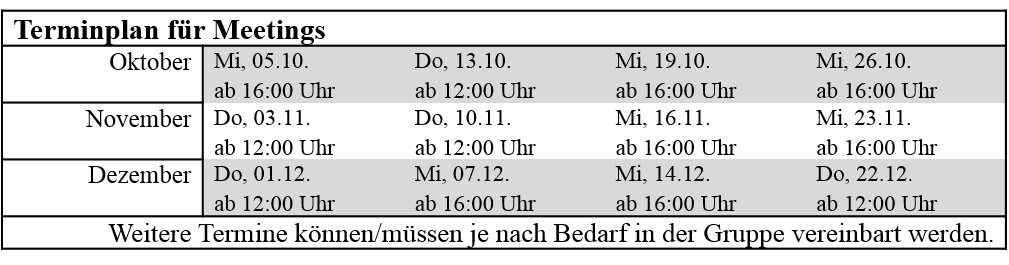
\includegraphics[scale=0.85]{images/Terminplan_Meetings.png}
\caption{Terminplan der Meetings}
\label{meets}
\end{figure}

\newpage

\subsection{Repository-Konzept}
Das Projekt wird mit dem Versionskontrollsystem Git verwaltet. Zentral wurde ein Repository auf GitHub angelegt. Erreichbar ist das Repository unter \url{https://github.com/mbutkereit/conveyor}. Änderungen werden lokal auf einem Branch vorgenommen, jedoch nicht auf dem Master. Sind die Änderungen erfolgreich abgeschlossen, kann der Master mit dem lokalen Branch zusammengeführt werden. Bevor ein push durchgeführt wird, muss gepullt werden. Nachdem ggf. Mergekonflikte gelöst wurden, kann vom Masterbranch aus auf das Repository gepusht werden.

\section{Projektmanagement}
Für die Gewährleistung eines guten Managements, werden in den folgenden Kapiteln erklärt wie die Teammitglieder mit ihren Aufgaben umgehen bzw. wann eine gegenseitige Benachrichtigung über ihren Fortschritt spätestens stattfinden sollte.

\subsection{Prozess}
Das Projekt wird auf Grundlage der geforderten Milestones umgesetzt. Für jede Implementierung ist zuvor ein geeignetes, sowie größtenteils selbsterklärendes bzw. verständliches, aber auch möglichst vollständiges Diagramm anzufertigen. Bestenfalls sollte die Visualisierung vor der Implementierung allen anderen Teammitgliedern vorgestellt werden, um mögliche Verbesserungen einzuholen und ggf. Konflikte früh zu erkennen sowie sie zu lösen. Die nachfolgende Tabelle \ref{visuals} listet für die jeweiligen Spezifikationen die im Team beschlossene Modellierung.

\begin{table}[h]
\center
\begin{tabularx}{\textwidth}{|l|X|}
\hline
\textbf{Spezifikation}&\textbf{Modellierung}\\
\hline
Codestruktur&UML Diagramm\\
\hline
Verhalten bzw. logische Abläufe&Zustandsautomat\\
\hline
Systemarchitektur&Komponentendiagramm\\
\hline
\end{tabularx}
\caption{Festgelegte Modellierung zur jeweiligen Spezifikation}
\label{visuals}
\end{table}

\subsection{PSP/Zeitplan/Tracking}
Zu jedem Praktikumstermin wird erwartet, dass die verteilten Aufgaben bzw. Milestones erfüllt werden. Um dies zu gewährleisten, muss jedes Teammitglied bei Schwierigkeiten andere Teammitglieder darüber sofort in Kenntnis setzen, damit frühzeitig ausgeholfen werden kann. Dazu wurden Arbeitspakete definiert und als Milestones in einem Gantt-Diagramm festgehalten.
\subsection{Qualitätssicherung}
Hinsichtlich der Qualitätssicherung, werden die vier Punkte Team, Modellierung, Code und Förderband herangezogen.
\medskip
\begin{compactenum}[1.]
\item \textbf{Team:} Jedes Teammitglied sollte über seine eigenen Fähigkeiten im Klaren sein und möglichst nur Aufgaben übernehmen, wofür es sich am besten geeignet fühlt. Darüber hinaus muss jedes Teammitglied bei Möglichkeit stets seine Unterstützung anbieten. Bei Problemen oder Überforderung müssen alle anderen Teammitglieder darüber unterrichtet und Aufgaben ggf. neu verteilt werden.
\medskip
\item \textbf{Modellierung:} Vor der Implementierung muss eine geeignete Visualisierung erstellt, anderen Teammitgliedern vorgestellt und diskutiert werden. 
\medskip
\item \textbf{Code:} Der Code wird nach beschlossenen Konventionen gefertigt. Dabei werden bekannte Pattern eingesetzt und verständliche sowie übersichtliche Realisierungen angestrebt. Den Maßstab hierfür setzen die Teammitglieder. Treten beim Code Review keine schwerwiegenden Anmerkungen bzw. Verständnisprobleme auf, gilt der Code als verständlich und übersichtlich.
\medskip
\item \textbf{Förderband:} Um hohen Durchsatz sowie Effizienz bei der Aussortierung zu erzielen, werden die Komponenten mit der höchstmöglichen Leistung für die jeweilige Situation angetrieben, während die Sicherheit des Bedieners im Vordergrund steht. Dabei werden Fehler- bzw. Ausnahmezustände ggf. durch einfache Signalcodes mithilfe der Ampel dem Bediener mitgeteilt.
\end{compactenum}

\section{Randbedingungen}
In diesem Kapitel werden die Bedingungen genannt unter denen das Projekt umgesetzt wird und die Mittel, die für die Umsetzung herangezogen werden.

\subsection{Entwicklungsumgebung}
Die drei Förderbänder werden über drei QNX Systeme gesteuert, die über eine serielle Schnittstelle verbunden sind. Als IDE wird QNX Momentics auf Windows 7 verwendet.

\subsection{Werkzeuge}
\begin{compactenum}[-]
\item QNX Momentics IDE 5.0
\item Latex(MiKTeX 2.9, Texmaker 4.5)
\item Git 2.8.1
\item Visual Paradigm 13.2
\item Gantt Project 2.8.1
\item Microsoft Visio 2016
\end{compactenum}

\subsection{Sprachen}
Das System wird in C++ 03 programmiert. Dabei werden vorgegebene Bibliotheken verwendet, welche in folgender Tabelle \ref{bibl} aufgelistet sind:
\medskip
\begin{table}[h]
\center
\begin{tabular}{|l|l|l|}
\hline
\textbf{Name}&\textbf{Version}&\textbf{Autor}\\
\hline
HWaccess.h&Unknown&Prof. Dr. Stephan Pareigis\\
\hline
HAWThread.h&Unknown&Prof. Dr. Stephan Pareigis \\
\hline
Lock.h&0.1&Simon Brummer \\
\hline
\end{tabular}
\caption{Verwendete Programmierbibliotheken}
\label{bibl}
\end{table}

\newpage

\section{Requirements and Use Cases}
Mithilfe der Requirements werden die Anforderungen an die einzelnen Komponenten des Förderbandes ermittelt. Dabei werden die Interessen der Stakeholder berücksichtigt.
\subsection{Stakeholder}
\begin{table}[h]
\center
\begin{tabularx}{\textwidth}{|X|X|}
\hline
\textbf{Stakeholder}&\textbf{Interessen}\\
\hline
Kunde&\begin{compactenum}[-]
      \item fehlerfreie Umsetzung der Anforderungen
      \item erfolgreiche Beendigung des Projektes 
      \end{compactenum}\\
\hline
Designer&\begin{compactenum}[-]
         \item übersichtliches, leicht erweiterbares Design
         \item sorgfältige Dokumentation 
         \end{compactenum}\\ 
\hline
Entwickler&\begin{compactenum}[-]
           \item präzises Design
           \item sinnvolle Kommentare
           \item lesbarer Code 
           \end{compactenum}\\
\hline
Tester&\begin{compactenum}[-]
       \item übersichtliches, vollständiges Testkonzept 
       \end{compactenum}\\
\hline
Bediener (Mitarbeiter, die das Laufband später bedienen sollen)&\begin{compactenum}[-]
\item einfache und intuitive Bedienung
\end{compactenum}\\
\hline
Instandhalter&\begin{compactenum}[-]
              \item robustes System
              \end{compactenum}\\
\hline
Andere Mitarbeiter&\begin{compactenum}[-]
                   \item Kenntnis über System und Funktionsweise
                   \end{compactenum}\\
\hline
\end{tabularx}
\caption{Stakeholder und ihre Interessen}
\label{stake}
\end{table}

\newpage

\subsection{Anforderungen}
\begin{table}[h]
\center
\begin{tabularx}{\textwidth}{|X|X|}
\hline
\textbf{Titel}&\textbf{Beschreibung}\\
\hline
Ansteuerung der Ampeln&Die Software soll die Ampel für folgende Fälle entsprechend ansteuern können:
\begin{compactenum}[-]
\item grünes Licht bei Normalbetrieb, fehlerfrei 
\item gelbes Licht bei Warnungen 
\item rotes Licht bei Fehler 
\end{compactenum}\\
\hline
Ansteuerung der Motoren der Förderbänder&Die Motoren der Förderbänder sollen in folgenden Varianten ansteuerbar sein: 
\begin{compactenum}[-]
\item Rechtslauf langsam/schnell
\item Linkslauf langsam/schnell
\item Stopp
\end{compactenum}\\
\hline
Ansteuerung der Weichen&Die Stellungen \su offen\so und \su geschlossen\so der Weichen müssen angesteuert werden. Außerdem soll beachtet werden, dass die Weichen nur für kurze Zeit die Stellung \su offen\so halten, um eine Beschädigung der Weichen zu vermeiden.\\
\hline
Erkennung von Werkstücken&Das System muss drei Arten von Werkstücke zuordnen können: 
\begin{compactenum}[-]
\item Flache Werkstücke 
\item Werkstücke mit Metalleinsatz (Bohrung liegt nach oben oder unten) 
\item Werkstücke ohne Metalleinsatz (Bohrung liegt nach oben oder unten)
\end{compactenum}\\
\hline
Aussortierung von Werkstücken&Flache Werkstücke und Werkstücke, bei der die Bohrung nach unten liegt, sollen aussortiert werden. \\
\hline
Reihenfolge der Werkstücke&Am Ende von Band 2 sollen die Werkstücke vereinzelt ankommen in der Reihenfolge:\hspace{2cm}
$\text{Bohrung oben ohne Metall}\rightarrow \text{Bohrung oben ohne Metall}\rightarrow \text{Bohrung oben mit Metall}$ \\
\hline
\end{tabularx}
\caption{Anforderungen(Teil 1)}
\label{anf1}
\end{table}

\newpage

\begin{table}[h]
\center
\begin{tabularx}{\textwidth}{|X|X|}
\hline
\textbf{Titel}&\textbf{Beschreibung}\\
\hline
Erkennung von Überschlagen der Werkstücke + Aussortierung des betreffenden Werkstücks&Das System soll erkennen, wenn sich Werkstücke bei der Übergabe von Band 1 zu Band 2 überschlagen und das betreffende Werkstück soll anschließend auf Band 2 aussortiert werden.\\
\hline
Langsamer Transport bei Höhenmessung&Wenn ein Werkstück durch die Höhenmessung transportiert wird, soll das Förderband langsam laufen.\\
\hline
Konsolenausgabe am Ende von Band 2&Wenn ein Werkstück das Ende von Band 2 erreicht, sollen auf der Konsole folgende Werkstückdaten ausgegeben werden:
\begin{compactenum}[-]
\item ID 
\item Typ 
\item Höhen-Messwert von Band 1 
\item Höhen-Messwert von Band 2 
\end{compactenum}\\
\hline
Konsolenausgabe am Ende von Band 3&Am Ende des dritten Bandes sollen die Werkstückdaten ankommender Werkstücke ausgegeben werden.\\
\hline
Stopp der Bänder bei keinen Werkstücken&Alle drei Bänder sollen jeweils stoppen, wenn sich kein Werkstück auf ihnen befindet.\\
\hline
Erkennung voller Rutschen&Volle Rutschen müssen mithilfe des Sensors am Rutscheneingang erkannt werden.\\
\hline
Rutschen koordinieren&Ist die Rutsche auf Band 1 voll, so soll die Aussortierung über Band 2 erfolgen. Umgekehrt, ist die Rutsche auf Band 2 voll, so soll die Aussortierung bereits auf Band 1 erfolgen.\\
\hline
Gebündelter Transport von Werkstückgruppen auf Band 3&Die drei sortierten Werkstücke sollen gebündelt (im Abstand von 1,5cm) an das Ende des dritten Bandes transportiert werden.\\
\hline
Fehlererfassung: Verschwinden von Werkstücken + Reaktion&Mittels Zeitmessung soll das Verschwinden von Werkstücken erfasst werden. Wenn zwischen zwei benachbarten Lichtschranken zuviel Zeit vergeht, in der kein Werkstück erfasst wurde, tritt folgende Reaktion auf: Bandstopp, Fehlermeldung.\\
\hline
\end{tabularx}
\caption{Anforderungen(Teil 2)}
\label{anf2}
\end{table}

\newpage

\begin{table}[h]
\center
\begin{tabularx}{\textwidth}{|X|X|}
\hline
\textbf{Titel}&\textbf{Beschreibung}\\
\hline
Fehlererfassung: Hinzufügen von Werkstücken + Reaktion&Mittels Zeitmessung soll das zu schnelle oder fehlerhafte Hinzufügen von Werkstücken erfasst werden. Wenn zwischen zwei benachbarten Lichtschranken die erwartete Zeit unterschritten wird, in der ein Werkstück erfasst werden müsste, dann tritt folgende Reaktion auf: Bandstopp, Fehlermeldung \\
\hline
Fehlererfassung: Beide Rutschen voll + Reaktion&Es soll erkannt werden, wenn beide Rutschen voll sind. Reaktion: Bandstopp, Fehlermeldung \\
\hline
\end{tabularx}
\caption{Anforderungen(Teil 3)}
\label{anf3}
\end{table}

\newpage
\subsection{Systemkontext}
Zum Systemkontext fallen Anforderungen aus Sicht der Software und des Systems an. Während bei der Software die Ansteuerung der Komponenten eines Förderbandes und die dazugehörigen Schnittstellen anfallen, ist aus Sicht der Systemebene die Kommunikation der Komponenten eines Förderbandes unter sich aber auch die der drei Förderbänder miteinander nötig. 

\subsubsection{Softwareebene}
Im Folgenden sind die Schnittstellen der Ereignisse aufgelistet, die zur Ansteuerung der einzelnen Komponenten ausgelöst sowie Ereignisse, die mithilfe der Sensoren erfasst werden. Die Methodennamen der erfassbaren Ereignisse beginnen mit \su is\so. 
\textbf{Port A (Ausgabeport)}
\begin{table}[h]
\center
\begin{tabularx}{\textwidth}{|X|X|}
\hline
\textbf{Ereignis}&\textbf{Methodenname}\\
\hline
Motor Rechtslauf&\begin{compactenum}[]
           \item \ttfamily right()
           \end{compactenum}\\
\hline
Motor Linkslauf&\begin{compactenum}[]
           \item \ttfamily left()
           \end{compactenum}\\
\hline
Motor langsam&\begin{compactenum}[]
           \item \ttfamily slow()
           \end{compactenum}\\
\hline
Motor schnell&\begin{compactenum}[]
           \item \ttfamily fast()
           \end{compactenum}\\
\hline
Motor Stopp&\begin{compactenum}[]
           \item \ttfamily stop()
           \end{compactenum}\\
\hline
Weiche auf/zu&\begin{compactenum}[]
           \item \ttfamily switchOpen()
           \item \ttfamily switchClosed()
           \end{compactenum}\\
\hline
Ampel Grün&\begin{compactenum}[]
           \item \ttfamily turnGreenOn()
           \item \ttfamily turnGrennOff()
           \end{compactenum}\\
\hline
Ampel Gelb&\begin{compactenum}[]
           \item \ttfamily turnYellowOn()
           \item \ttfamily turnYellowOff()
           \end{compactenum}\\
\hline
Ampel Rot&\begin{compactenum}[]
           \item \ttfamily turnRedOn()
           \item \ttfamily turnRedOff()
           \end{compactenum}\\
\hline
\end{tabularx}
\caption{API auf Port A(Ausgabeport) - auslösbare Ereignisse}
\label{portA}
\end{table}

\newpage

\noindent\textbf{Port B (Eingabeport)}
\begin{table}[h]
\center
\begin{tabularx}{\textwidth}{|X|X|}
\hline
\textbf{Ereignis}&\textbf{Methodenname}\\
\hline
Einlauf Werkstück&\begin{compactenum}[]
           \item \ttfamily isItemRunningIn()
           \end{compactenum}\\
\hline
Werkstück in Höhenmessung&\begin{compactenum}[]
           \item \ttfamily isItemAltimetry()
           \end{compactenum}\\
\hline
Höhenmessung&\begin{compactenum}[]
           \item \ttfamily isItemInAltimetryToleranceRange()
           \end{compactenum}\\
\hline
Werkstück in Weiche&\begin{compactenum}[]
           \item \ttfamily isItemSwitch()
           \end{compactenum}\\
\hline
Werkstück Metall&\begin{compactenum}[]
           \item \ttfamily isItemMetal()
           \end{compactenum}\\
\hline
Weiche offen&\begin{compactenum}[]
           \item \ttfamily isSwitchOpen()
           \end{compactenum}\\
\hline
Rutsche voll&\begin{compactenum}[]
           \item \ttfamily isSkidFull()
           \end{compactenum}\\
\hline
Auslauf Werkstück&\begin{compactenum}[]
           \item \ttfamily isItemRunningOut()
           \end{compactenum}\\
\hline
\end{tabularx}
\caption{API auf Port B (Eingabeport) - erfassbare Ereignisse}
\label{portB}
\end{table}

\newpage

\noindent\textbf{Port C (Ein-/Ausgabeport)}
\begin{table}[h]
\center
\begin{tabularx}{\textwidth}{|X|X|}
\hline
\textbf{Ereignis}&\textbf{Methodenname}\\
\hline
LED Starttaste&\begin{compactenum}[]
           \item \ttfamily turnLedStartOn()
           \item \ttfamily turnLedStartOff()
           \end{compactenum}\\
\hline
LED Resettaste&\begin{compactenum}[]
           \item \ttfamily turnLedResetOn()
           \item \ttfamily turnLedResetOff()
           \end{compactenum}\\
\hline
LED Q1&\begin{compactenum}[]
           \item \ttfamily turnLedQ1On()
           \item \ttfamily turnLedQ1Off()
           \end{compactenum}\\
\hline
LED Q2&\begin{compactenum}[]
           \item \ttfamily turnLedQ2On()
           \item \ttfamily turnLedQ2Off()
           \end{compactenum}\\
\hline
Taste Start&\begin{compactenum}[]
           \item \ttfamily isButtonStartPressed()
           \end{compactenum}\\
\hline
Taste Stopp&\begin{compactenum}[]
           \item \ttfamily isButtonStopPressed()
           \end{compactenum}\\
\hline
Taste Reset&\begin{compactenum}[]
           \item \ttfamily isButtonResetPressed()
           \end{compactenum}\\
\hline
Taste E-Stopp&\begin{compactenum}[]
           \item \ttfamily isButtonEStopPressed()
           \end{compactenum}\\
\hline
\end{tabularx}
\caption{API auf Port C (Ein-/Ausgabeport) - auslösbare/erfassbare Ereignisse}
\label{portC}
\end{table}

\newpage

\subsubsection{Systemebene}
Die nachfolgende Abbildung \ref{syskont} visualisiert die Systemgrenzen der Förderbandanlage. Dabei sind die dazugehörigen Sensoren und Aktoren abgebildet durch welche eine Förderbandanlage mit der Umwelt und seiner Nachbarsysteme kommuniziert. Die Tabellen \ref{senstasks} und \ref{acttasks} listen die Aufgaben der Sensoren und Aktoren auf.

\begin{figure}[h]
\hspace{-1.2cm}
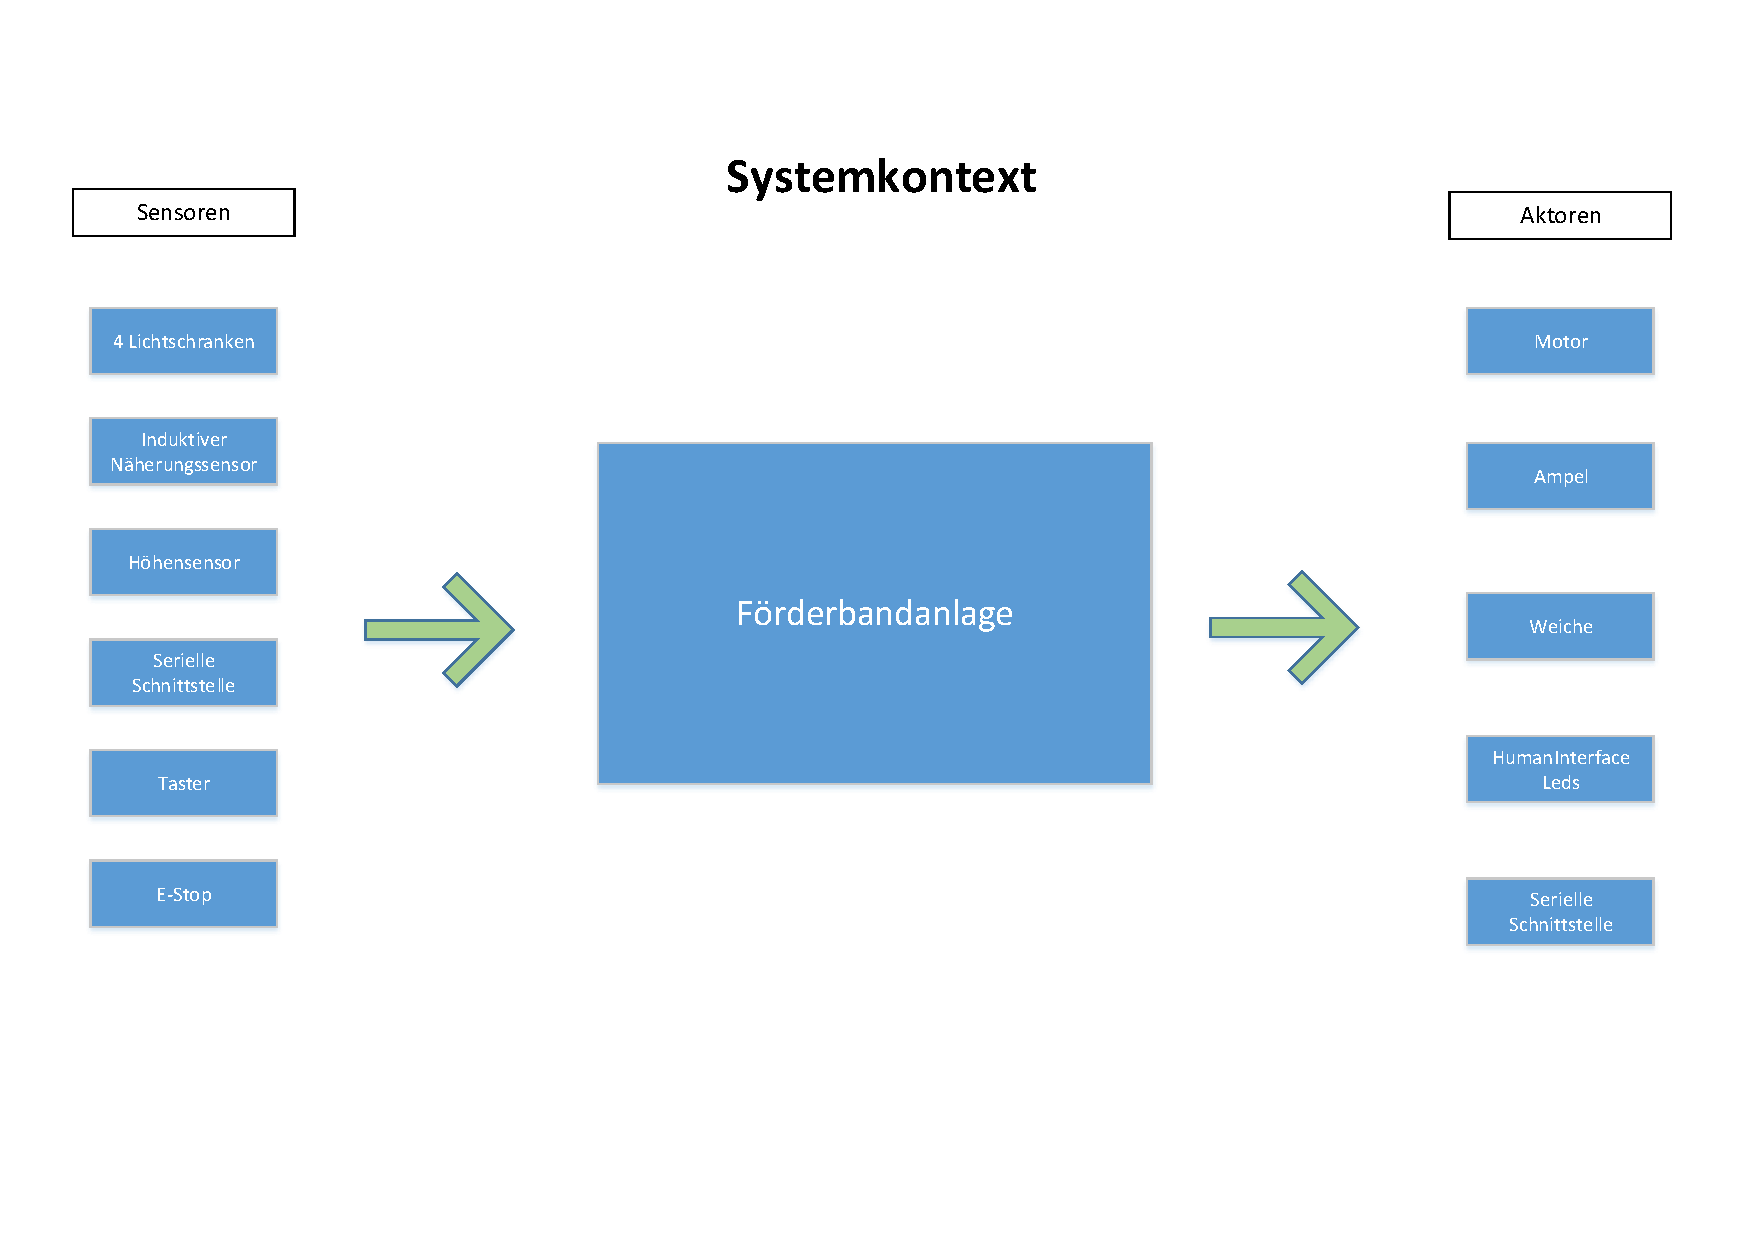
\includegraphics[scale=0.6]{images/Systemkontext.pdf}
\caption{Systemgrenzen der Förderbandanlage mit Sensoren und Aktoren}
\label{syskont}
\end{figure}

\begin{table}[h]
\center
\begin{tabularx}{\textwidth}{|l|X|}
\hline
\textbf{Sensor}&\textbf{Aufgabe}\\
\hline
4 Lichtschranken&Erfassen, ob sich gerade ein Werkstück sich auf der Höhe der jeweiligen Lichtschranke befindet.\\
\hline
Induktiver Näherungssensor&Stellt fest, ob es sich um ein metallisches Werkstück handelt.\\
\hline
Höhensensor&Misst die Höhe des Werkstücks.\\
\hline
Serielle Schnittstelle&Ermöglicht den Empfang von Datenpaketen anderer Nachbarsysteme.\\
\hline
Taster&Löst je nach Programmierung entsprechende Aktion aus.\\
\hline
E-Stop&Schaltet alle Förderbänderbänder bedingungslos aus.\\
\hline
\end{tabularx}
\caption{Sensoren und deren Aufgaben}
\label{senstasks}
\end{table}

\begin{table}[h]
\center
\begin{tabularx}{\textwidth}{|l|X|}
\hline
\textbf{Aktor}&\textbf{Aufgabe}\\
\hline
Motor&Treibt das band der Förderbandanlagen an.\\
\hline
Ampel&Signalisiert entsprechend anliegender Ereignisse.\\
\hline
Weiche&Sortiert bei falscher Reihung Werkstücke aus.\\
\hline
HumanInterface Leds&Signalisieren dem Bediener Sensorereignisse\\
\hline
Serielle Schnittstelle&Ermöglicht das Versenden von Datenpaketen an andere Nachbarsysteme\\
\hline
\end{tabularx}
\caption{Aktoren und deren Aufgaben}
\label{acttasks}
\end{table}

\newpage

\subsection{Use Cases}

\begin{table}[h]
\center
\begin{tabularx}{\textwidth}{X}

\begin{compactenum}[1.]
\item \textbf{Flache Werkstücke aussortieren}
\medskip

Akteure: Mitarbeiter (legt die Werkstücke auf das Band), Höhenmessung, Weiche
\medskip

Auslösendes Ereignis: Höhenmessung erkennt das flache Werkstück.
\medskip

Kurzbeschreibung: Die flachen Werkstücke werden auf Band 1 mit der Höhenmessung erkannt und über die Weiche aussortiert.
\bigskip

\item \textbf{Werkstückdaten ausgeben}
\medskip

Akteure: Lichtschranke, Display
\medskip

Auslösendes Ereignis: Die Lichtschranke auf Band 2 wird durchquert.
\medskip

Kurzbeschreibung: Wenn ein Werkstück das Ende von Band 2 erreicht, werden die Werkstückdaten auf dem Display ausgegeben.
\bigskip

\item \textbf{Ausgabe der Werkstücke auf Band 3 in der richtigen Reihenfolge}
\medskip

Akteure: Lichtschranke, Mitarbeiter (nimmt die Werkstücke in Empfang), Weiche
\medskip

Auslösendes Ereignis: Es sind die drei richtigen Werkstücke auf Band 3 vorhanden.
\medskip

Kurzbeschreibung: Auf Band 3 werden jeweils 3 Werkstücke gebündelt in der richtigen Reihenfolge ($\text{Bohrung oben ohne Metall}\rightarrow \text{Bohrung oben ohne Metall}\rightarrow \text{Bohrung oben mit Metall}$) ausgegeben.
\end{compactenum}
\end{tabularx}
%\caption{Tabellenunterschrift}
\label{ucs}
\end{table}

\newpage

\section{Design}
Im Designentwurf sind Systemarchitektur, Datenmodellierung und Verhaltensmodellierung der Förderbänder enthalten.

\subsection{Systemarchitektur}
Die Systemarchitektur setzt sich aus den internen Architekturen der drei Förderbänder und der Architektur des Gesamtsystems, welche die Schnittstellen der drei Förderbänder zueinander darstellt, zusammen.

\subsubsection{Förderband intern}

\begin{figure}[h]
\centering 
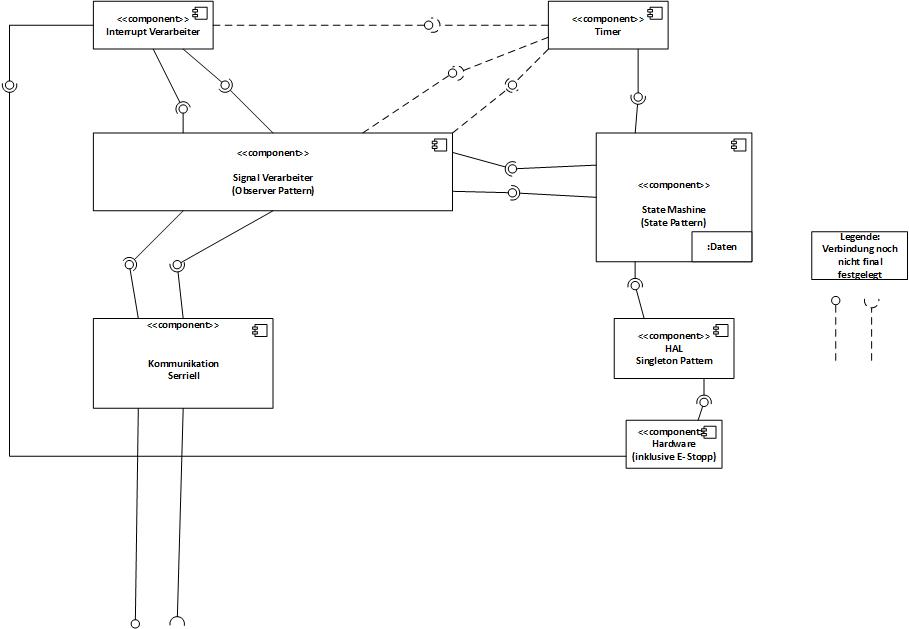
\includegraphics[scale=0.7]{images/SW_Architektur/Foerderband.jpg}
\caption{Interne Systemarchitektur eines Förderbandes}
\label{archintern}
\end{figure}

\begin{table}[h]
\center
\begin{tabularx}{\textwidth}{|l|X|}
\hline
\textbf{Komponente}&\textbf{Aufgabe}\\
\hline
Interrupt Verarbeiter&Verarbeitet Interrupts aus Timer, Signal Verarbeiter und Hardware.\\
\hline
Timer&Zeiterfassung für zeitkritische Abläufe.\\
\hline
Signal Verarbeiter&Verarbeitet Signale aus Interrupt Verarbeiter, Timer, Statemachine und Kommunikation seriell.\\
\hline
Statemachine&Steuert den logischen Ablauf.\\
\hline
Kommunikation seriell&Bildet die Schnittstelle zwischen Förderband und Gesamtsystem.\\
\hline
HAL&Hardwareabstraktionsschicht zur Ansteuerung der Komponenten eines Förderbandes.\\
\hline
Hardware&Hardware des Förderbandes\\
\hline
\end{tabularx}
\caption{Aufgaben der Komponenten eines Förderbandes}
\label{archinterntcomp}
\end{table}

\newpage

\subsubsection{Gesamtsystem}

\begin{figure}[h]
\centering 
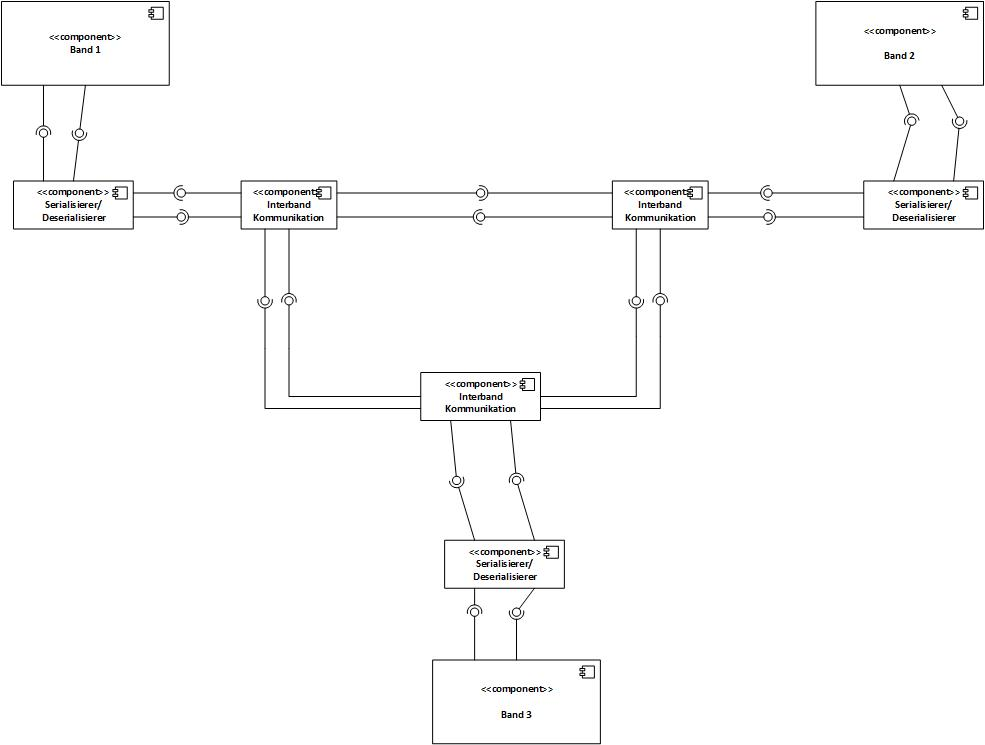
\includegraphics[scale=0.60]{images/SW_Architektur/Gesamtsystem.jpg}
\caption{Systemarchitektur des Gesamtsystems}
\label{archtotal}
\end{figure}

\begin{table}[h]
\center
\begin{tabularx}{\textwidth}{|l|X|}
\hline
\textbf{Komponente}&\textbf{Aufgabe}\\
\hline
Band 1&Erstes Förderband, welches die Sortierung entsprechend der Reihung durchführt.\\
\hline
Band 2&Zweites Förderband, welches die Sortierung entsprechend der Reihung durchführt.\\
\hline
Band 3&Drittes Förderband, welches die Gruppierung der Werkstücke übernimmt und anschließend übergibt.\\
\hline
Serialisierer/Deserialisierer&Serialisiert bzw. deserialisiert Datenpakete zur Kommunikation.\\
\hline
Interband Kommunikation&Empfängt bzw. versendet serialisierte Datenpakete.\\
\hline
\end{tabularx}
\caption{Aufgaben der Komponenten des Gesamtsystems}
\label{archtotalcomp}
\end{table}

\newpage

\subsection{Datenmodellierung}
Die Modellierung der Klassen und dessen Methoden sind mithilfe von UML-Diagrammen realisiert.
\subsubsection{HAL}
Mit Der Klasse HAL werden die Hardwarekomponenten eines Förderbandes angesteuert. Dabei wird jede Hardwarekomponente nach dem Singleton-Pattern instanziiert. Die nachfolgende Abbildung \hyperref[sec:umlhal]{5} stellt alle Klassen zur HAL mit ihren Methoden dar.
\newpage

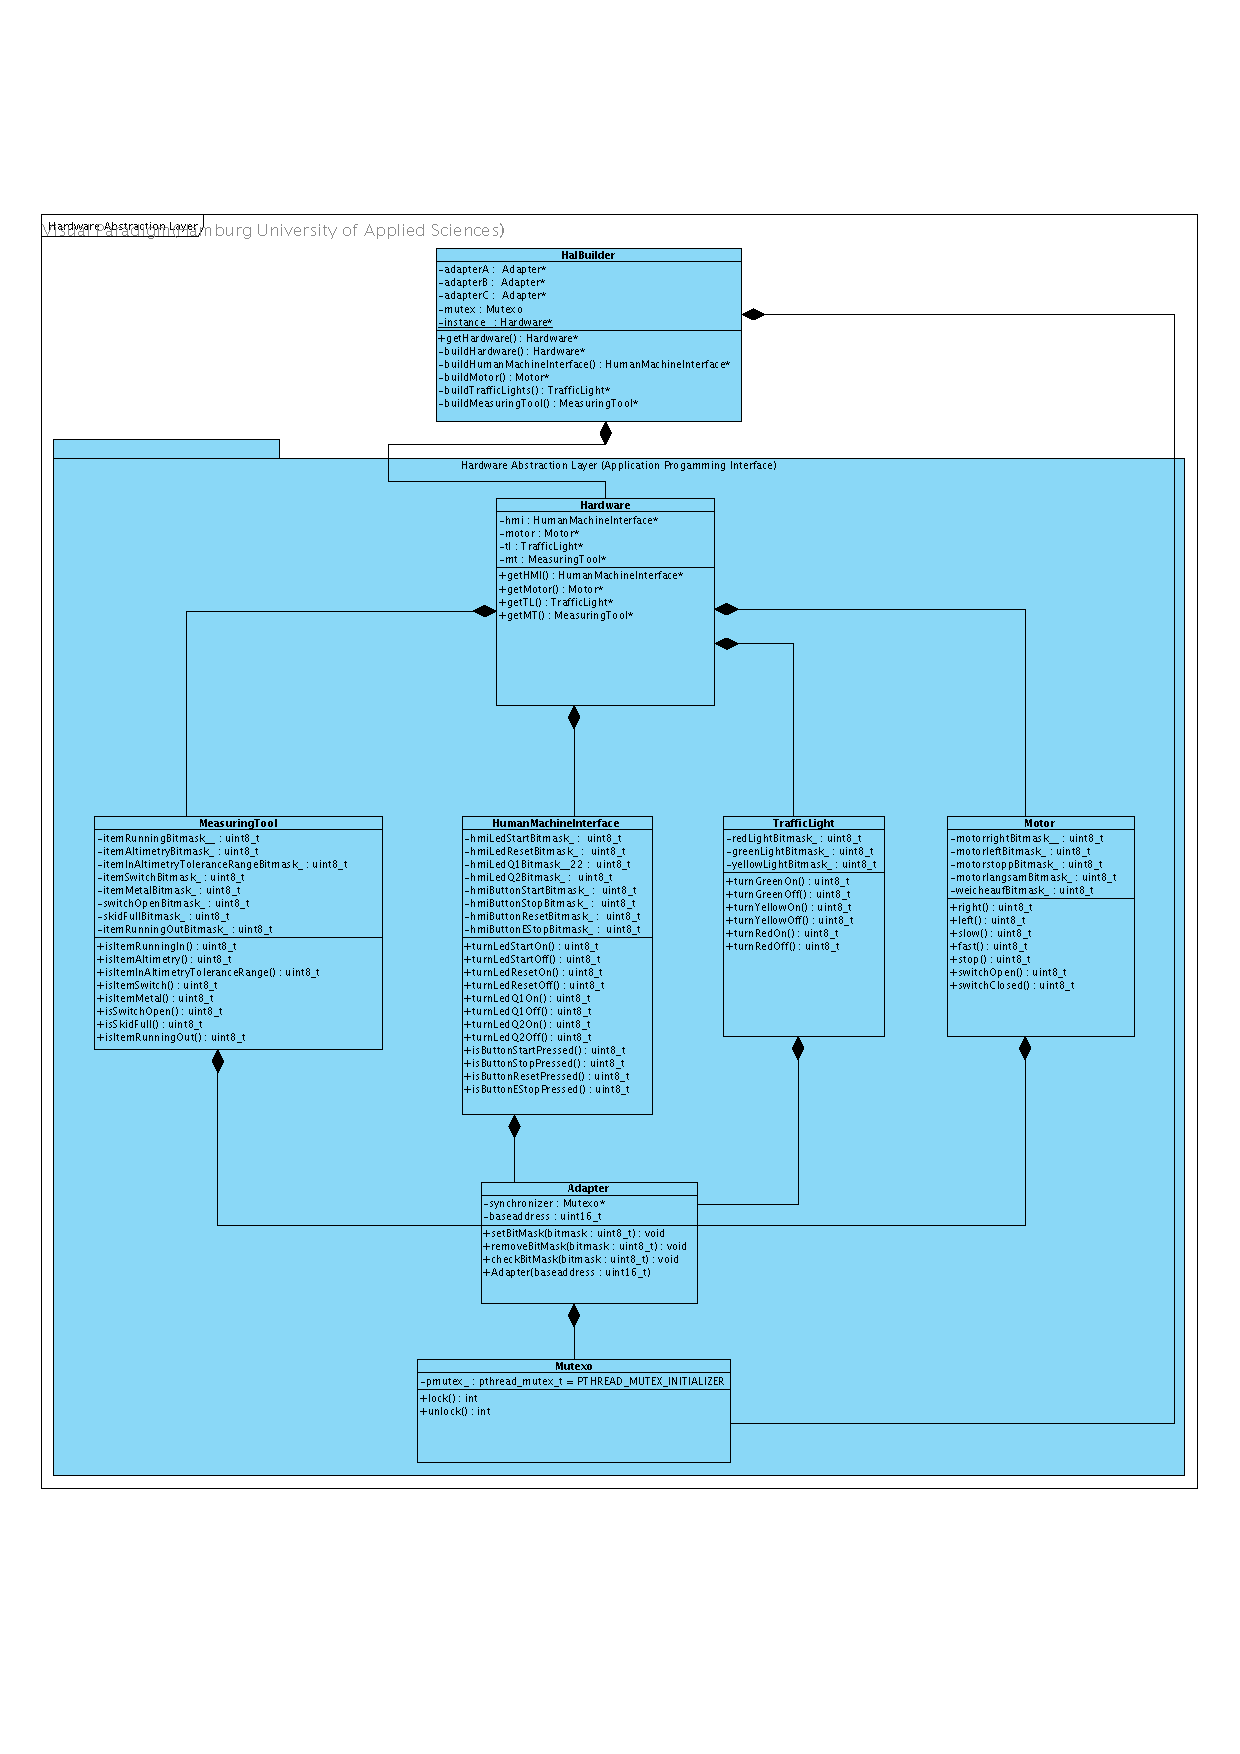
\includepdf[scale=1,pages=1,offset=0 50, pagecommand=
\vspace*{21.5cm}
\hspace*{3cm} Abbildung 5: UML-Diagramm zur HAL]{images/HAL_UML.pdf}\label{sec:umlhal}
\newpage

\subsection{Zeitmessung}
Auf allen Förderbändern muss jeweils eine Zeitmessung durchgeführt werden, um Zeiten zu erfassen, mit denen im Normalbetrieb unsachgemäß hinzugefügte Werkstücke oder das Verschwinden von Werkstücken erkannt werden kann.

\subsubsection{Vorbedingungen}
Für die Zeitmessung muss eine ähnliche Routine laufen, die auch im Normalbetrieb für die Förderbänder ablaufen wird, wobei Messvorgänge ausgelassen werden und ggf. das Werkstück bedingungslos durchgelassen wird. Falls in der Routine Geschwindigkeitsänderungen des Bandes vorliegen, müssen diese jedoch miteinbezogen werden, nur die aktive Messung nicht.
Da das Band der jeweiligen Förderbänder nicht perfekt geführt wird und der Timer eine relativ hohe Zeitauflösung hat, müssen \textbf{best} und \textbf{worst case} Zeiten ermittelt werden. 

\subsubsection{Ausführung}
Für den \textbf{\textcolor{ForestGreen}{best case}} wird das Werkstück beim Hinzufügen von der ersten Lichtschranke aus gesehen am \textbf{\textcolor{ForestGreen}{linken Rand}} der Führung angelegt, während beim \textbf{\textcolor{OrangeRed}{worst case}} am \textbf{\textcolor{OrangeRed}{rechten Rand}} angelegt werden muss. Dabei muss das Werkstück die erste Lichtschranke auch unterbrechen, was trivialerweise auch im Normalbetrieb beim Hinzufügen weiterer Werkstücke beachtet werden muss! Die Zeitmessung beginnt, nachdem das Werkstück die Lichtschranke am Anfang nicht mehr unterbricht. Unterbricht das Werkstück die nachfolgenden Lichtschranken, wird jeweils die Zeit gestoppt. Die nachfolgende Abbildung \hyperref[sec:Messpunkte]{6} zeigt wann die Zeiten $t_0, t_H, t_W$ und $t_E$ erfasst werden.

\begin{figure}[h]
\centering 
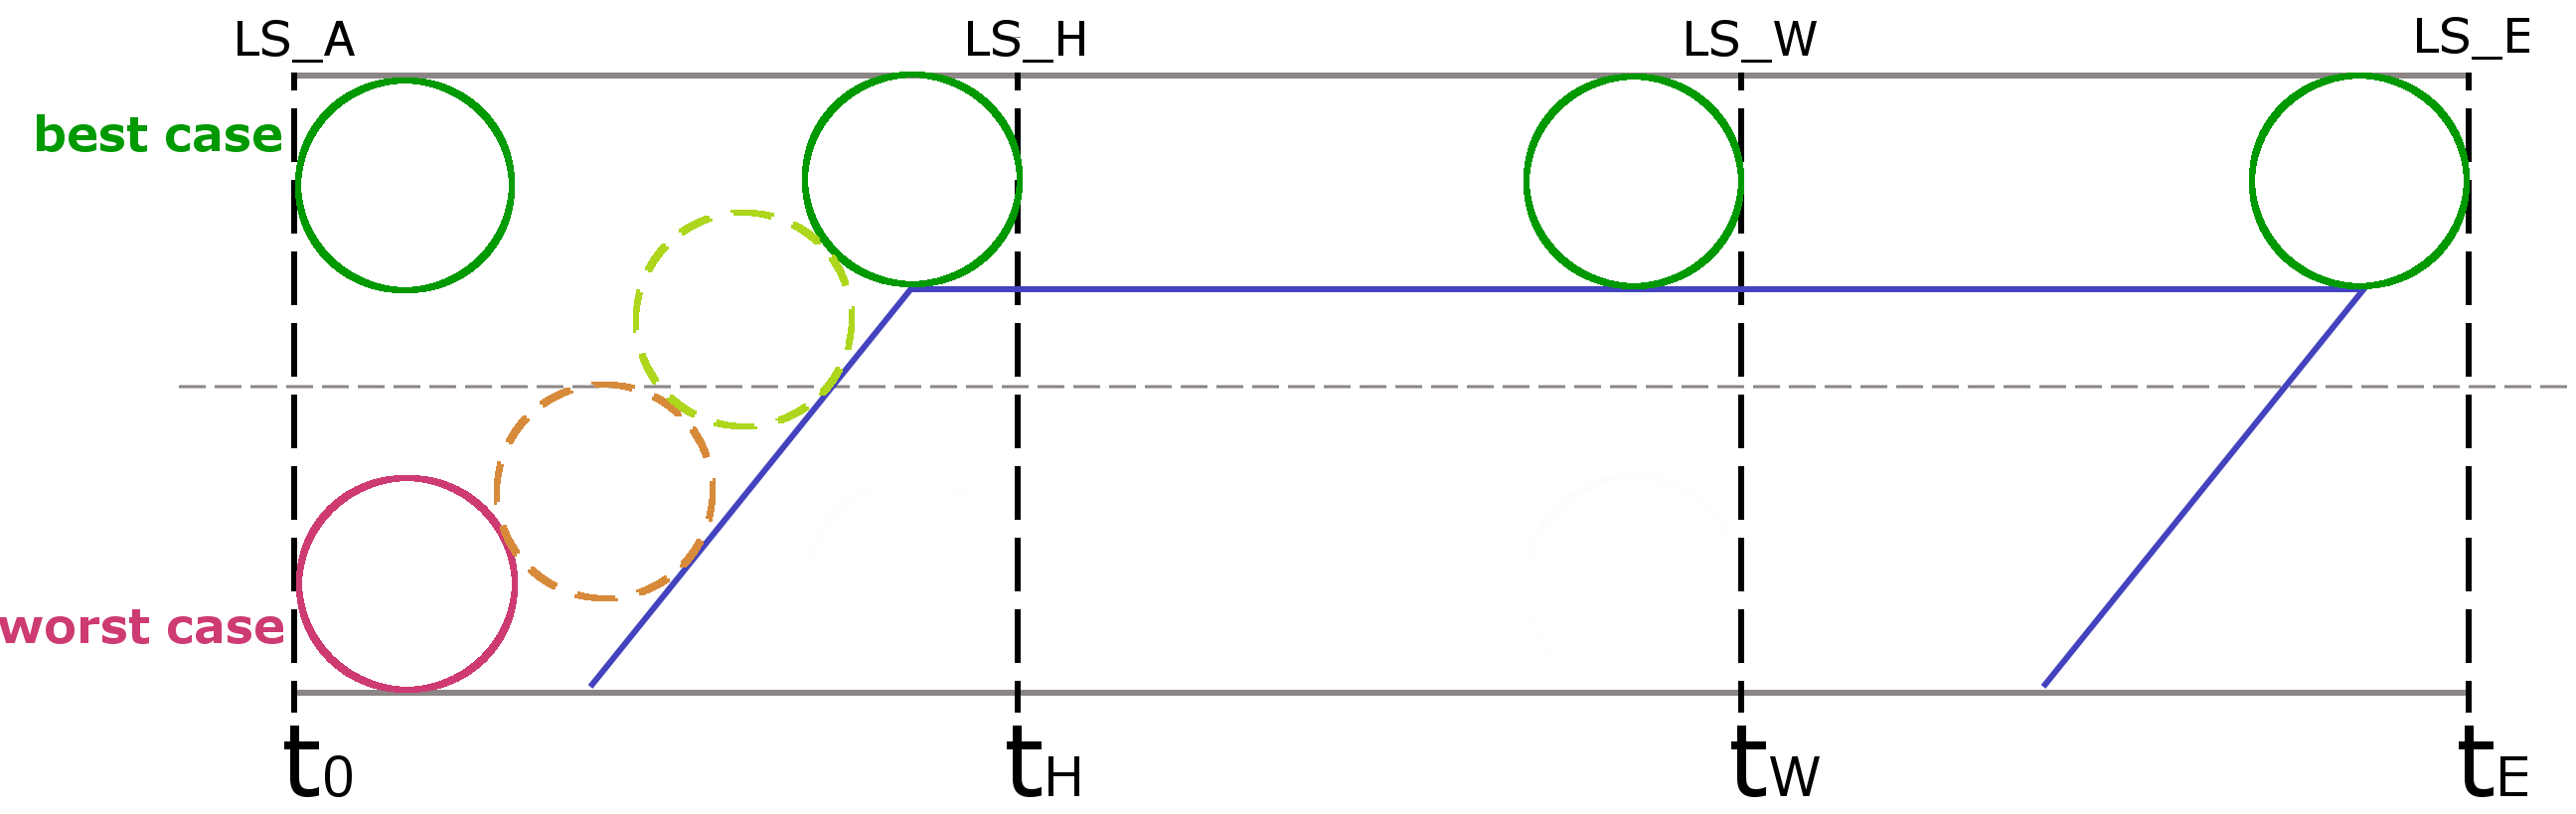
\includegraphics[scale=0.6]{images/Zeitmessung_Platzierung.png}
\caption*{Abbildung 6: Stoppen der Zeit an den Lichtschranken: \textit{LS\_A, LS\_H, LS\_W, LS\_E}}
\label{sec:Messpunkte}
\end{figure}
\noindent \textit{LS\_A}: Lichtschranke-Anfang, 
\textit{LS\_H}: Lichtschranke-Höhenmessung, 
\textit{LS\_W}: Lichtschranke-Weiche, 
\textit{LS\_E}: Lichtschranke-Ende.\\

\noindent Auf der nachfolgenden Seite ist der endliche Automat in Abbildung \hyperref[sec:timemeasure]{7} zur Zeitmessung abgebildet.

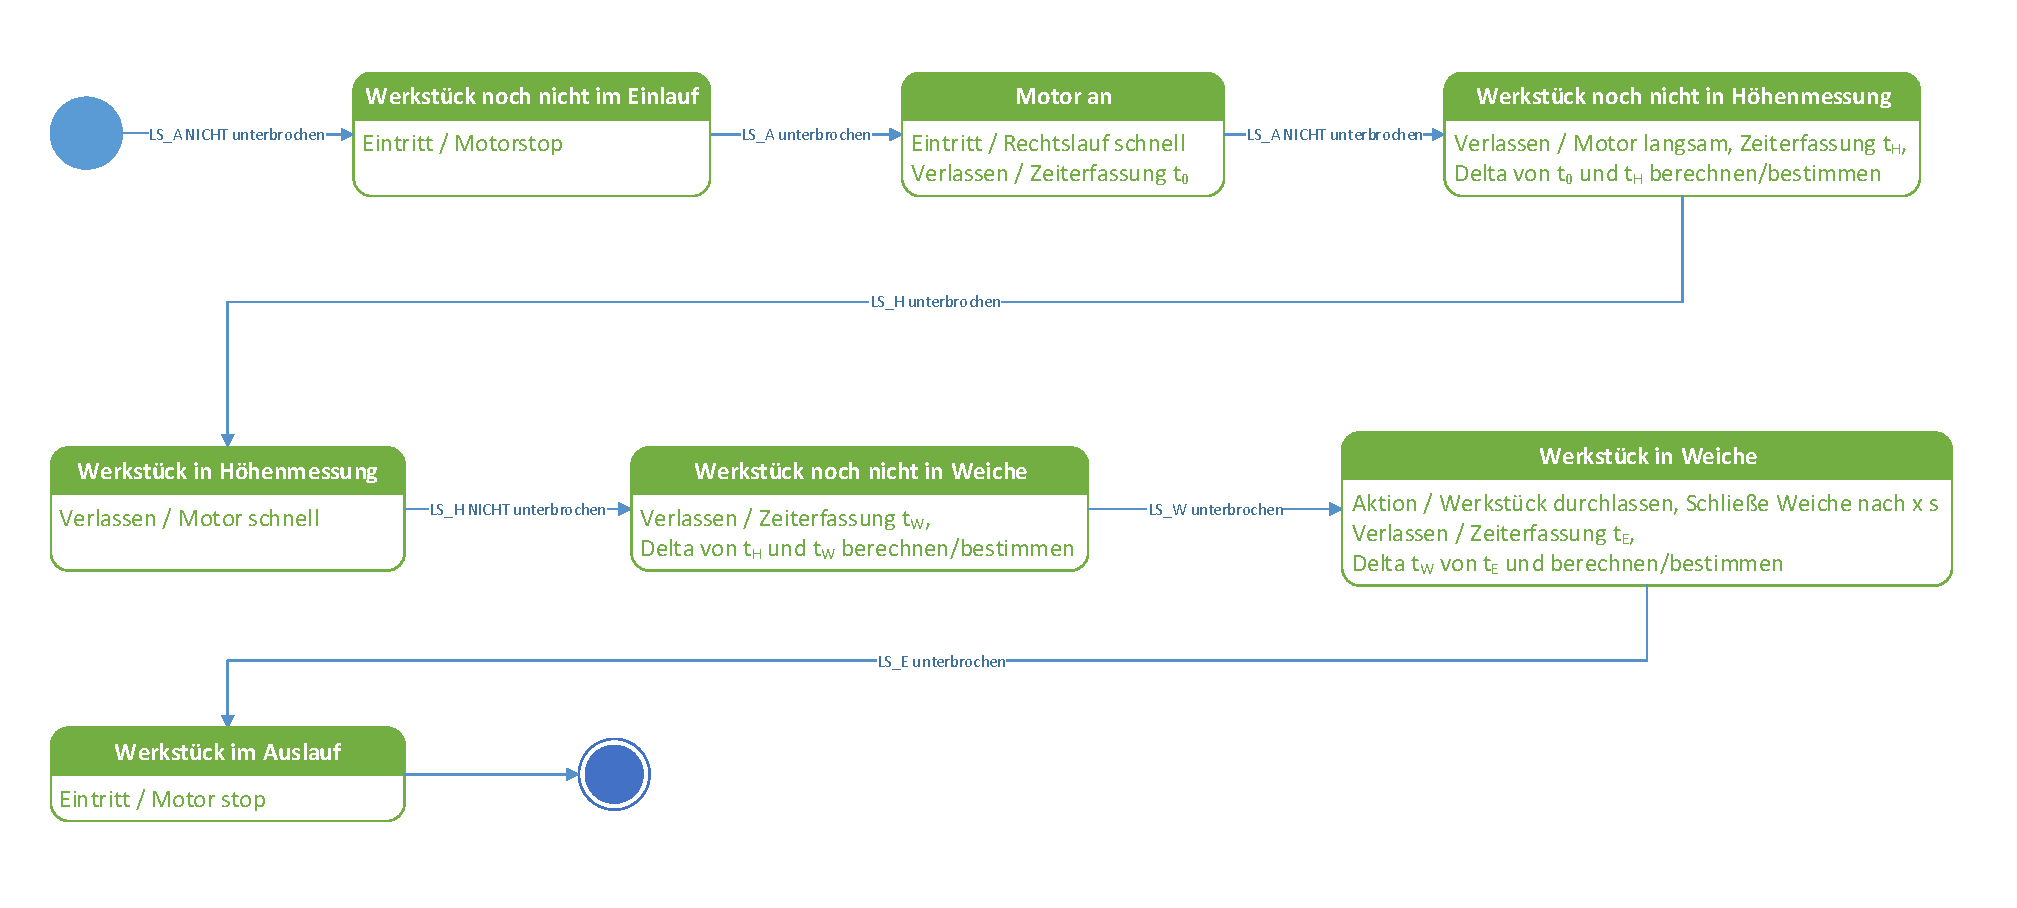
\includepdf[scale=0.9,pages=1, landscape=true, offset=0 20, pagecommand=
\vspace*{25cm}
\hspace*{3cm} Abbildung 7: FSM zur Zeitmessung]{images/Zeitmessung_FSM.pdf}\label{sec:timemeasure}

\newpage

\subsection{Verhaltensmodellierung}
Das Verhalten der drei Förderbänder ist mithilfe von hierarchischen Zustandsautomaten realisiert. Nach der Durchführung einer Zeitmessung, sind alle drei Förderbänder bereit für den Normalbetrieb. Die Abbildungen \hyperref[sec:hsm1]{8}, \hyperref[sec:hsm2]{9} und \hyperref[sec:hsm3]{10} auf den folgenden Seiten bilde die Förderbänder 1, 2 und 3 ab.

\newpage

\includepdf[scale=0.87,pages=2, landscape=true, offset=0 13, pagecommand=
\vspace*{25cm}
\hspace*{3cm} Abbildung 8: HSM zu Förderband 1]{FSM/Statemachines.pdf}\label{sec:hsm1}

\newpage

\includepdf[scale=0.86,pages=4, landscape=true, offset=0 15, pagecommand=
\vspace*{24.9cm}
\hspace*{3cm} Abbildung 9: HSM zu Förderband 2]{FSM/Statemachines.pdf}\label{sec:hsm2}

\newpage

\includepdf[scale=0.86,pages=6, landscape=true, offset=0 13, pagecommand=
\vspace*{24.9cm}
\hspace*{3cm} Abbildung 10: HSM zu Förderband 3]{FSM/Statemachines.pdf}\label{sec:hsm3}

\newpage
\section{Implementierung}
\textcolor{red}{Anmerkung: Nur wichtige Implementierungsdetails sollen hier erklärt werden. Code-Beispiele (snippets) können hier aufgelistet werden, um der Erklärung zu dienen. 
Anmerkung: Bitte KEINE ganze Programme hierhin kopieren!
}

\section{Testen}
Das Testen der Förderbänder findet nach Fertigstellung von Milestones statt, welche die Ansteuerung der Förderbänder sowie deren Kommunikation untereinander enthalten. Die Tests reichen von essentiellen Ansteuerungstests einzelner Komponenten der Förderbänder bis hin zur Ablaufsteuerung über alle drei Bänder. Für die Abnahme werden speziell komplexere Tests durchgeführt.

\subsection{HAL der Aktorik}
\begin{table}[h]
\center
\begin{tabularx}{\textwidth}{|l|X|X|X|}
\hline
\textbf{ID}&\textbf{Funktion}&\textbf{Test erfolgreich}&\textbf{Anmerkung}\\
\hline
1&Rote Lampe an&Ja&\\
\hline
2&Rote Lampe aus&Ja&\\
\hline
3&Gelbe Lampe an&Ja&\\
\hline
4&Gelbe Lampe aus&Ja&\\
\hline
5&Grüne Lampe an&Ja&\\
\hline
6&Grüne Lampe aus&Ja&\\
\hline
7&Motor langsam&Ja&\\
\hline
8&Motor schnell&Ja&\\
\hline
9&Motor links&Ja&\\
\hline
10&Motor rechts&Ja&\\
\hline
11&Motor stoppen&Ja&\\
\hline
12&Weiche auf&Ja&\\
\hline
13&Weiche zu&Ja&\\
\hline
14&Led Start an&Ja&\\
\hline
15&Led Start aus&Ja&\\
\hline
16&Led Reset an&Ja&\\
\hline
17&Led Reset aus&Ja&\\
\hline
18&Led Q1 an&Ja&\\
\hline
19&Led Q1 aus&Ja&\\
\hline
20&Led Q2 an&Ja&\\
\hline
21&Led Q2 aus&Ja&\\
\hline
\end{tabularx}
\caption{Testauswertung zur HAL der Aktorik}
\label{tstg1}
\end{table}

\subsection{HAL der Sensorik}
\textcolor{red}{Hier erscheinen bald die Tests zu der HAL der Sensorik sowie deren Auswertung.}

\subsection{Serielle Schnittstelle}
\textcolor{red}{Hier erscheinen bald die Tests zu der seriellen Schnittstelle sowie deren Auswertung.}

\subsection{Anlagensteuerung pro Band}
\textcolor{red}{Hier erscheinen bald die Tests zur Anlagensteuerung pro Band sowie deren Auswertung.}

\subsection{Ablaufsteuerung über alle drei Bänder}
\textcolor{red}{Hier erscheinen bald die Tests zur Ablaufsteuerung über alle drei Bänder sowie deren Auswertung.}

\subsection{Testkonzept für die Abnahme} 
\begin{table}[h]
\center
\begin{tabularx}{\textwidth}{|l|X|X|X|}
\hline
\textbf{ID}&\textbf{Funktion}&\textbf{Test erfolgreich}&\textbf{Anmerkung}\\
\hline
1&Erkennung der Werkstücke am Anfang des Förderbandes&&\\
\hline
2&Flache Werkstücke werden aussortiert&&\\
\hline
3&Bei der Aussortierung der flachen Werkstücke blinkt die gelbe Leuchte&&\\
\hline
4&Werkstücke mit der Bohrung nach unten werden aussortiert&&\\
\hline
5&Bei Förderband 1, Fehlermeldung bei voller Rutsche&&\\
\hline
6&Bei Förderband 2, Fehlermeldung und Stopp von Förderband 1 und Förderband 2 bei voller Rutsche&&\\
\hline
7&Stopp beim leeren Förderband&&\\
\hline
8&Beim Verschwinden von Werkstücken wird eine Fehlermeldung ausgegeben und das Förderband stoppt&&\\
\hline
9&Beim Hinzufügen von Werkstücken mitten auf dem Förderband wird eine Fehlermeldung ausgegeben und das Förderband stoppt&&\\
\hline
10&Am Ende von Band 2 soll die gewünschte Reihenfolge der Werkstücke entstehen&&\\
\hline
\end{tabularx}
\caption{Testauswertung der Abnahmetests(Teil 1)}
\label{tstl1}
\end{table}

\newpage

\begin{table}[h]
\center
\begin{tabularx}{\textwidth}{|l|X|X|X|}
\hline
\textbf{ID}&\textbf{Funktion}&\textbf{Test erfolgreich}&\textbf{Anmerkung}\\
\hline

12&Am Ende vom Band 3 werden die Werkstückdaten als 3er Gruppe ausgegeben auf der Konsole&&\\
\hline
13&Förderband 3 transportiert die Werkstücke erst dann bis zum Ende des Bandes wenn die 3er Gruppe vollständig ist.&&\\
\hline
\end{tabularx}
\caption{Testauswertung der Abnahmetests(Teil 2)}
\label{tstl2}
\end{table}

\section{Lessons Learned}
\textcolor{red}{Führen sie ein Teammeeting durch in dem gesammelt wird, was gut gelaufen war, was schlecht gelaufen war und was man im nächsten Projekt (z.B. im PO) besser machen will. Listen sie für die Aspekte jeweils mindestens drei Punkte auf. Weitere Erfahrungen und Erkenntnisse können hier ebenso kommentiert werden, auch Anregungen für die Weiterentwicklung des Praktikums.}

\section{Anhang}

\subsection{Glossar}
\textcolor{red}{Eindeutige Begriffserklärungen}

\subsection{Abkürzungen}
\textcolor{red}{Listen sie alle Abkürzungen auf, die sie in diesem Dokument benutzt haben.}

\end{document}

% Weitere Syntax für verschiedene Anwendungsfelder

%Aufzählungen
%\begin{compactenum}[1.]
%\item
%\end{compactenum}

%\ref{labelname des zu Referenzierenden Objekts}

%Tabelle
%\begin{table}[h]
%\center
%\begin{tabular}{|l|l|}
%\hline
%\textbf{linke Spaltenüberschrift}&\textbf{rechte Spaltenüberschrift}\\
%\hline
%1&2\\
%\hline
%3&4\\
%\end{tabular}
%\caption{Zugriffsoperationen}
%\label{labelname}
%\end{table}

%Tabelle mit tabularx
%\begin{table}[h]
%\center
%\begin{tabularx}{\textwidth}{|l|X|}
%\hline
%Text in linker Spalte&Text in rechter Spalte der über den Rand hinausragt\\
%\hline
%\end{tabularx}
%\caption{Tabellenunterschrift}
%\label{labelname}
%\end{table}

%Grafik einfügen
%\begin{figure}[h]
%\centering 
%\includegraphics[scale=0.3]{Dateiname}
%\caption{Bildunterschrift}
%\label{labelname}
%\end{figure}

%Linksbündig mit definierter Einrückung
%\begin{flushleft}
%\leftskip0.6cm
%\end{flushleft}

%Codelisting
%\lstset{basicstyle=\ttfamily}
%\begin{lstlisting}
%Code
%\end{lstlisting}

%Erzeugen eines Inhaltsverzeichnisses und ihrer Einträge
%\tableofcontents
%\section{•}
%\subsection{•}

%Vertikaler Abstand
%\vspace{0cm}

%Etwas zentrieren
%\centering 

%Um PDFs skaliert einzufügen und Seitenzahl sowie header beizubehalten 
%\includepdf[pages={2}, nup=1x1, scale=0.9, pagecommand={}]{file.pdf}

%Um PDFs ohne Skalierung einzufügen und Seitenzahl sowie header beizubehalten 
%\label{labelname}\hypertarget{haluml}{}
%\includepdf[pages=1,pagecommand={}]{file.pdf}

%Um PDFs einfach einzufügen, Seitenzahl, header und footer werden überlagert
%\includepdf[landscape=true,pages=-]{file.pdf}

%Um PDFs mit vorangehendem Text einzufügen mit Skalierung
%\includepdf[scale=0.8,pages=1,pagecommand=\subsection{Kapitel} Text]{file.pdf}

%Literaturverzeichnis anlegen
%\bibliography{Literaturverzeichnis}